\section{Strmentazione}
	In qest'esperienza esperienza sono state impiegate :
	\begin{itemize}
		\item 2 circiti integrati SN7400 sati per costitire i circiti in esame
		\item varie resistenze e capacità impiegateanch'esse per il montaggio dei circiti
		\item 1 DIP switch a 4 interrttori
		\item 1 diodo 1N418
		\item 2 diodi LED, impiegati per rendere osservabile visivamente le tabelle di verità. 
		\item Il circito implsatore basato sl Ardino nano montato nell'esperienza n:10
		\item n mltimetro digitale
		\item oscilloscopio digitale 
		\item n generatore di fnzioni
	\end{itemize}
\section{verifica tabella NEND}
	Per la verifica della tabella di verità di na porta NEND \tablename{ \ref{t:NEND}}
	\begin{table}[htb]
		\centering
		\begin{tabular}{|s|s|s|}
				\toprule
				\text{ingresso} A & \text{ingresso} B &\text{scita porta NAND }$\overline{A\cdot B}$	\\
				\midrule
				0  & 0 & 1\\
				0  & 1 & 1\\
				1  & 0 & 1\\
				1  & 1 & 0\\
				\bottomrule
			\end{tabular}
			\caption{Tabella di verità di na porta NEND.}
			\label{t:NEND}
		\end{table}
	si è procedto in de maniere distinte; na prima verifica visiva che impiega il DIP switch in dotazione; ed na che impiega il circito implsatore basato s ardino.
	Per entrambi i modi si è montato il circito in \figurename{ \ref{f:NEND}}
	\begin{figure}[htb]
		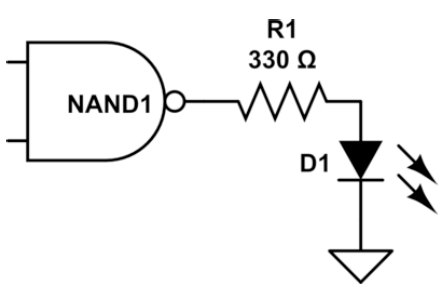
\includegraphics[scale=1.0]{../immagini/NEND.png}
	\end{figure}\label{f:NEND}